
	\begin{figure}[H]
		\centering
		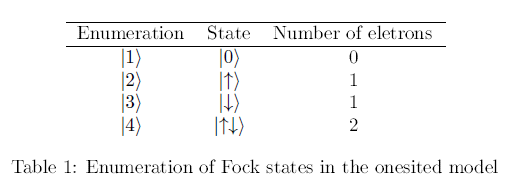
\includegraphics[width=0.3\linewidth]{states} \qquad \qquad 
		\caption{Different states in the Hilbert space in two different notations}
		\label{fig1}
	\end{figure}
\section{Explicit solution of the 2-site model}
For the $N=2$ half-filled Hubbard model with periodic boundary the exact calculation of correlation functions is doable "by hand" because the Hilbert space contains only six states ($\ket{\phi_J}$, $J=1,...,6$), thus the trace can be performed explicitly. Figure \ref{fig1} shows the states in operator-notation and a shorthand notation. One sees that e.g. for $\ket{\phi_1}$ there is a sign ambiguity in defining the state
\begin{align*}
	\ket{\phi_1^a} &= c^{\dagger}_{1\uparrow}c^{\dagger}_{0\uparrow}\ket{0} \\
	\ket{\phi_1^b} &= c^{\dagger}_{0\uparrow}c^{\dagger}_{1\uparrow}\ket{0} = -\ket{\phi_1^a} 
\end{align*}
where the creation operator indices are for lattice site 0 and 1 and spin up and down. Due to this ambiguity we choose the convention that lattice sites increase from right to left and for same lattice sites spin up are on the right to spin down operators.\\ Writing down the Hubbard Hamiltonian for the 2 site model in the basis of these six states gives a $6x6$ matrix\footnote{note that the problem reduces to a 4x4 and two 1x1 matrices due to the conservation of total spin.}
\begin{equation*}
	H=
\begin{pmatrix}
	0 & 0 & 0&0&0&0\\
	0 & U & -t&-t&0&0\\
	0 & -t & 0&0&-t&0\\
	0 & -t & 0&0&-t&0\\
	0 & 0 & -t&-t&U&0\\
	0 & 0 & 0&0&0&0 
\end{pmatrix}
\end{equation*}
The goal is to calculate expectation values of an operator $A$ in the canonical ensemble
\begin{equation}
	<A> = \frac{\text{Tr}(\text{e}^{-\beta H}A)}{\text{Tr}(\text{e}^{-\beta H})} = \frac{\sum_{n}^{}\text{e}^{-\beta E_n}\braket{\tilde{\phi_n}|A|\tilde{\phi_n}}}{\sum_{n}^{}\text{e}^{-\beta E_n}}\label{expvalue}
\end{equation}
where $E_n$ are the eigenenergies and $\ket{\tilde{\phi_n}}$ are the eigenstates of $H$. Diagonalizing $H$ gives the 4x4 matrix 
\begin{equation*}
H_D=
\begin{pmatrix}
0 & 0 & 0&0\\
0 & U & 0&0\\
0 & 0 & E_{-}&0\\
0 & 0 & 0&E_{+}
\end{pmatrix}
\end{equation*}
where $E_{\pm}=\frac{1}{2}(U\pm\sqrt{16t^2+U^2})$, along with the set of eigenstates.\footnote{$\ket{\phi_1}$ and $\ket{\phi_6}$ are also eigenstates of H}
\begin{align*}
	\tilde{\phi_{0}}&=-\ket{\phi_3}+\ket{\phi_4}+\ket{\phi_5}\\
	\tilde{\phi_{U}}&=-\ket{\phi_2}+\frac{E_+}{2t}\ket{\phi_4}+\frac{E_-}{2t}\ket{\phi_5}	\\
	\tilde{\phi_{-}}&=\ket{\phi_2}+\frac{E_+}{2t}\ket{\phi_4}+\frac{E_-}{2t}\ket{\phi_5}	\\
	\tilde{\phi_{+}}&=\ket{\phi_3}+\ket{\phi_4}+\ket{\phi_5}	
\end{align*}
With this one can calculate for instance the energy expectation value 
\begin{equation}
	<E>  = \frac{\sum_{n}^{}\text{e}^{-\beta E_n}E_n}{\sum_{n}^{}\text{e}^{-\beta E_n}}
\end{equation}
or the propagator according to equation \ref{expvalue}.
\begin{equation}
	<c^{\dagger}_{i\sigma}c_{j\sigma^{\prime}}>= \frac{\sum_{n}^{}\text{e}^{-\beta E_n}\braket{\tilde{\phi_n}|c^{\dagger}_{i\sigma}c_{j\sigma^{\prime}}|\tilde{\phi_n}}}{\sum_{n}^{}\text{e}^{-\beta E_n}}
\end{equation}

